%!TEX root = ../my_thesis.tex


\ifthenelse{\equal{\templateVersion}{UBX}}
{
\appendix

\chapter{Compléments au Chapitre 1}
\section{Détails 1}\label{append:decoding_nodes}
}
{
%%
%%  Annexes
%%
%%  Note: Ne pas modifier la ligne ci-dessous. / Do not modify the following line.
\ifthenelse{\equal{\Langue}{english}}{
	\addcontentsline{toc}{compteur}{APPENDICES}
}{
	\addcontentsline{toc}{compteur}{ANNEXES}
}
%%
%%
%%  Toutes les annexes doivent être inclues dans ce document
%%  les unes à la suite des autres.
%%  All annexes must be included in this document one after the other.
\Annexe{COMPL\'EMENTS AU CHAPITRE 1}
\label{append:decoding_nodes}
}

Les sorties du canal composite sont des informations souples données par le démodulateur.
Ce bruit additif est ajouté à la valeur des données en sortie du modulateur $\mathbold{x}$.
\begin{equation}
y_i = x_i + n_i
\end{equation}
Dans le modèle de chaine de communication considéré, la puissance du bruit du canal AWGN $N_0$ est supposée connue.
Cela permet au démodulateur de calculer la probabilité conditionnelle suivante.
\begin{equation}
	P_r( \tilde{y}_i|\tilde{x}_i) = \dfrac{1}{\sqrt{\pi N_0}}\exp^{-\tfrac{(\tilde{x}_i^2-\tilde{y}_i^2)}{N_0}}
\end{equation}
$p_i$ représente la probabilité de recevoir $\tilde{y}_i$ en présupposant la valeur de $\tilde{x}_i$ en sortie du modulateur ($\tilde{x}_i=-1$ ou $\tilde{x}_i=1$). Les \textit{likelihood ratios} (LRs), sont exprimés en fonction de ces probabilités :
\begin{equation}
	l_i = \log\left(\dfrac{P_r(y_i | x_i = 0)}{P_r(y_i | x_i = 1)}\right)
\end{equation}
\label{eq:lr}

Les \textit{log likelihood ratios} (LLR), sont le logarithme népérien des LR ! 

\begin{equation}
  L_i = \log\left(\dfrac{P_r(y_i | x_i = 0)}{P_r(y_i | x_i = 1)}\right)
\end{equation}
\label{eq:llr}


Les codes correcteurs d'erreurs peuvent être définis par un ensemble de contraintes de parités. Une représentation graphique de ces contraintes est appelé \textit{graphe de Tanner} comme représenté en Figure~\ref{fig:noeuds}.

\begin{figure}[t]
\centering
\includegraphics{tail/appendix_1_fig/noeuds}
\caption{Représentations des noeuds de décodage}
\label{fig:noeuds}
\end{figure}

Le noeud de parité est la représentation graphique de l'équation suivante : 
\begin{equation}
b_0 + b_1 + b_2 = 0
\end{equation}
Tandis que l'encodeur canal associe le vecteur d'entrée $\mathbold{b}$ de longueur $K$ à un mot de code $\mathbold{x}$ de longueur $N$, le décodeur combine les différents LR ou LLR en sortie du canal composite dans le but de retrouver les bits d'origine.
Dans l'exemple de la Figure~\ref{fig:noeuds}, les estimations du canal pour les valeurs des bits $b_1$ et $b_2$, notés respectivement $l_1$ et $l_2$, peuvent être combinées afin de calculer une estimation extrinsèque du bit $b_0$, notée $l_0^e$.

Sa valeur est par définition :
\begin{equation}
l^e_0 = \dfrac{P(y_1,y_2 | b_0 = 0)}{P(y_1,y_2 | b_0 = 1)}
\label{eq:le0}
\end{equation}
Seules deux combinaisons possibles des bits $b_1$ et $b_2$ peuvent impliquer que $b_0$ soit égal à $0$ : ou bien $b_1=0$ et $b_2=0$, ou bien $b_1=1$ et $b_2=1$. Il est donc possible de calculer $P(b_0|y_1,y_2)$ : 
\begin{equation}
P(y_1,y_2 | b_0 = 0)  =  P(y_1 | b_1 = 0)P(y_2 | b_2 = 0) + P(y_1 | b_1 = 1)P(y_2 | b_2 = 1) \\
\end{equation}
Donc,  
\begin{equation}
P(y_1,y_2 | b_0 = 0)  =  l_1l_2 + 1 \\
\label{eq:le1}
\end{equation}


De la même manière,
\begin{equation}
P(b_0 = 1 | y_1,y_2) =P(y_1 | b_1 = 0)P(y_2 | b_2 = 1) + P(y_1 | b_1 = 1)P(y_2 | b_2 = 0)
\end{equation}
Donc, 
\begin{equation}
P(b_0 = 1 | y_1,y_2) = l_1 + l_2
\label{eq:le2}
\end{equation}
On déduit donc de \ref{eq:le0}, \ref{eq:le1} et \ref{eq:le2} : 

\begin{equation}
l^e_0=\dfrac{1 + l_1l_2}{l_1+l_2}
\label{eq:parity}
\end{equation}

En effectuant la même démarche pour le N\oe{}ud d'égalité il est possible d'obtenir :
\begin{eqnarray*}
\begin{array}{r c l}
P(y_1,y_2|b_0=0) & = & P(y_1|b_1=0) P(y_2 | b_2 = 0) \\
P(y_1,y_2|b_0=1) & = & P(y_1|b_1=1) P(y_2 | b_2 = 1) 
\end{array}
\end{eqnarray*}
Il est possible d'en déduire l'extrinsèque :
\begin{equation}
l^e_0=l_1l_2
\label{eq:equality}
\end{equation}

L'algorithme de décodage SC peut être représenté sous la forme de \textit{factor graph} dans lequel les équations \ref{eq:parity} et \ref{eq:equality} sont appliquées, comme montré en Figure~\ref{fig:SCSchedule}. Les fonctions élémentaires F et G sont des combinaisons des équations liées aux \noeuds de parité et aux \noeuds d'égalités.
\begin{figure}[t]
  \centering
  \subfloat[][$F$ function]{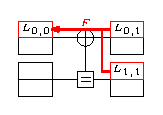
\includegraphics[width=.24\textwidth]{tail/appendix_1_fig/SC_graph2_b}}\quad\quad\quad\quad
  \subfloat[][$G$ function]{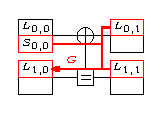
\includegraphics[width=.25\textwidth]{tail/appendix_1_fig/SC_graph2_d}}
  \caption{Fonctions $F$ et $G$ de l'algorithme SC}
  \label{fig:SCSchedule}
\end{figure}
\begin{equation}
l_{0,0} = F(l_{0,1}, l_{1,1}) = \dfrac{1+l_{0,1}l_{1,1}}{l_{0,1}+l_{1,1}}
\end{equation}
\[
	l_{1,0} = 
	\begin{cases} 
	l_{1,1}l_{0,1} & \text{if }S_{0,0} = 0\\
	l_{1,1}\dfrac{1}{l_{0,1}} & \text{if }S_{0,0} = 1
	\end{cases}
\]
Cela peut être simplifié : 
\begin{equation}
l_{1,0} = G(l_{1,1},l_{0,1},S_{0,0}) = l_{1,1}l_{0,1}^{1 - 2S_{0,0}}
\end{equation}

Ces équations utilisent des LR. Elles peuvent être modifiées afin de faire apparaître les LLR : 

\begin{equation}
L_{0,0} = f(L_{0,1}, L_{1,1}) = 2\tanh^{-1}(\tanh(L_{0,1})\tanh(L_{1,1}))
\end{equation}
\begin{equation}
L_{1,0} = g(L_{1,1},L_{0,1},S_{0,0}) = L_{1,1} + (1 - 2S_{0,0})L_{0,1}
\end{equation}

Enfin, $f$ peut être simplifiée \cite{fossorier1999reduced} : 
\begin{equation}
f(L_{0,1}, L_{1,1}) \approx \text{sign}(L_{0,1})\text{sign}(L_{1,1})\text{min}(|L_{0,1}|,|L_{1,1}|))
\end{equation}